% ============================ Part 1: GenAI & LLMs ============================
\section{Part 1 $\cdot$ Generative AI \& LLMs}

\newcommand{\genaiList}[1]{%
\begin{itemize}\setlength{\itemsep}{6pt}\color{#1}
  \item \textbf{Text \& chat:} ChatGPT, Claude, Gemini, Llama, Qwen, DeepSeek
  \item \textbf{Code:} GitHub Copilot, Cursor, Claude Code
  \item \textbf{Images / video:} Stable Diffusion, Midjourney, Sora, Veo
  \item \textbf{Multimodal:} one model reads images, audio, and text
  \item \textbf{Agents:} LLMs that browse, call tools, write and run code
\end{itemize}}

\begin{frame}{Generative AI is everywhere (2026)}
\begin{columns}[T]
\begin{column}{0.4\textwidth}
\vspace{6pt}
\genaiList{black}
\end{column}
\begin{column}{0.58\textwidth}
\centering
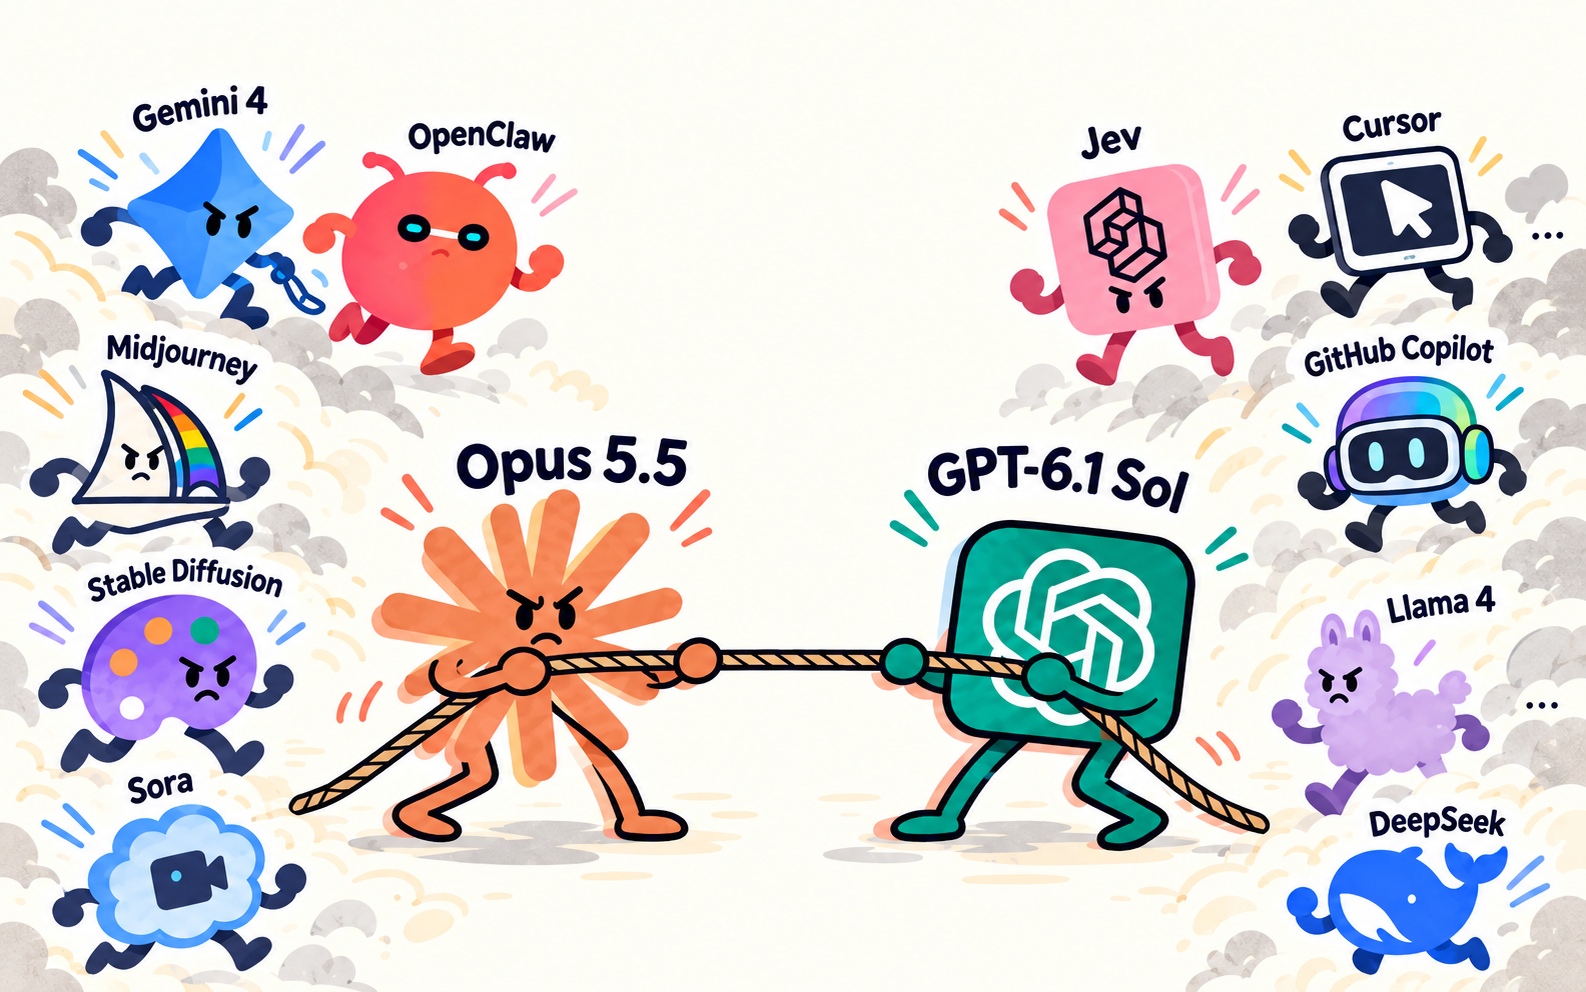
\includegraphics[width=\textwidth,height=0.66\textheight,keepaspectratio]{figs/frontier_tug_of_war.png}\\[2pt]
{\small A new frontier model every few months.}\\
{\scriptsize\color{midgray} (illustration generated with ChatGPT)}
\end{column}
\end{columns}
\end{frame}

\begin{frame}{Generative AI is everywhere (2026)}
\begin{columns}[T]
\begin{column}{0.46\textwidth}
\vspace{6pt}
\genaiList{midgray}
\end{column}
\begin{column}{0.52\textwidth}
\vspace{10pt}
\begin{tcolorbox}[enhanced,colback=uvanavy!6,colframe=uvanavy,boxrule=1pt,arc=3pt,left=8pt,right=8pt,top=8pt,bottom=8pt]
\raggedright
\textbf{Behind all of it:}\\[6pt]
the \textbf{Transformer} (\href{https://arxiv.org/abs/1706.03762}{Vaswani et al., 2017})\\[3pt]
$+$ \textbf{self-supervised pretraining}\\ \hspace*{1.2em}{\small(on trillions of words of web text)}\\[3pt]
$+$ \textbf{scale}\\[3pt]
$+$ \textbf{mid- and post-training}\\ \hspace*{1.2em}{\small(fine-tuning, alignment, RL)}\\[8pt]
\textcolor{uvaorange!85!black}{\textbf{We will focus on the last one today.}}
\end{tcolorbox}
\end{column}
\end{columns}
\end{frame}

\begin{frame}{Discriminative vs.\ generative: an LLM is both}
\begin{center}
\begin{tikzpicture}[font=\small,>=Latex,node distance=6mm]
  \node[draw,rounded corners,fill=softgray,minimum width=2.6cm,minimum height=0.8cm,align=center] (x1) {image / features $x$};
  \node[draw,rounded corners,fill=uvanavy!10,right=of x1,minimum height=0.8cm,minimum width=1.6cm] (m1) {model};
  \node[draw,rounded corners,fill=softgray,right=of m1,minimum height=0.8cm,text width=4.3cm,align=center] (y1) {label $y$\\\scriptsize a class (``cat'') or a number (3.7)};
  \draw[->,thick] (x1) -- (m1); \draw[->,thick] (m1) -- (y1);
  \node[anchor=south,text=uvanavy] at ($(x1.west)!0.5!(y1.east) + (0,0.5)$) {so far in this course: learn $p(y\mid x)$};
  \node[draw,rounded corners,fill=softgray,minimum width=2.6cm,minimum height=0.8cm,align=center,below=12mm of x1] (x2) {prompt $x$};
  \node[draw,rounded corners,fill=uvaorange!15,right=of x2,minimum height=0.8cm,minimum width=1.6cm] (m2) {LLM};
  \node[draw,rounded corners,fill=softgray,right=of m2,minimum height=0.8cm,text width=4.3cm,align=center] (y2) {text $y$\\\scriptsize a paragraph or a piece of code};
  \draw[->,thick] (x2) -- (m2); \draw[->,thick] (m2) -- (y2);
  \node[anchor=south,text=uvaorange!80!black] at ($(x2.west)!0.5!(y2.east) + (0,0.5)$) {today: learn $p(\text{text})$, then \emph{sample}};
\end{tikzpicture}
\end{center}
\begin{itemize}\setlength{\itemsep}{4pt}
  \item A classifier picks one of $K$ labels.
  \item A generative model puts probability on \emc{whole pieces of data} and can produce new ones.
  \item An LLM is \emc{both}: a classifier over the next word, run in a loop to generate text.
\end{itemize}
\end{frame}

\begin{frame}{Zooming out: the machine learning timeline}
\begin{center}
\begin{tikzpicture}[font=\footnotesize,>=Latex,
  era/.style={signal,signal to=east,signal from=west,fill=uvaorange!80,text=white,font=\footnotesize\bfseries,
              minimum height=1.05cm,text width=1.45cm,align=center,inner xsep=2pt},
  lab/.style={text width=1.85cm,align=center,font=\scriptsize,anchor=north}]
  \node[era,signal from=nowhere] (e1) at (0,0) {1950s--60s};
  \node[era,right=1mm of e1] (e2) {70s--80s};
  \node[era,right=1mm of e2] (e3) {90s};
  \node[era,right=1mm of e3] (e4) {2000s};
  \node[era,right=1mm of e4] (e5) {2010s};
  \node[era,right=1mm of e5,fill=uvanavy] (e6) {2023--now};
  \node[lab] at ([yshift=-3mm]e1.south) {the start; neural nets first become popular};
  \node[lab] at ([yshift=-3mm]e2.south) {rule-based and knowledge-based systems};
  \node[lab] at ([yshift=-3mm]e3.south) {CNNs and RNNs invented};
  \node[lab] at ([yshift=-3mm]e4.south) {classic ML: SVMs, random forests, Bayesian nets};
  \node[lab] at ([yshift=-3mm]e5.south) {ImageNet; deep learning breakthroughs};
  \node[lab,text=uvanavy,font=\scriptsize\bfseries] at ([yshift=-3mm]e6.south) {ChatGPT, generative AI, agentic AI};
  \node[above=4mm of e6,text=uvaorange!85!black,font=\small\bfseries,align=center] (today) {today};
  \draw[->,very thick,uvaorange!85!black] (today.south) -- (e6.north);
\end{tikzpicture}
\end{center}
\vspace{4pt}
\keybox{\textbf{The core has not changed.} Today's models are still \emc{neural networks trained by gradient descent on a loss}, exactly what you learned in the first half of this course. What changed is the \emc{architecture}, the \emc{data}, the \emc{scale}, and the \emc{training recipe}.}
\end{frame}

\begin{frame}{Zooming in: 2017 to 2026}
\begin{center}
\begin{tikzpicture}[font=\scriptsize,>=Latex]
  \draw[very thick,uvanavy,->] (0.0,0) -- (13.1,0);
  \foreach \x/\yr/\lab/\part/\side in {
    0.7/2017/{Transformer\\``Attention is all you need''}/{}/1,
    2.15/2018/{GPT-1, BERT\\pretrain, then fine-tune}/{Parts 2, 4}/-1,
    3.6/2019/{GPT-2 (1.5B)\\coherent long text}/{Part 2}/1,
    5.05/2020/{GPT-3 (175B)\\in-context learning}/{Part 3}/-1,
    6.5/2022/{ChatGPT\\RLHF alignment}/{Parts 5--6}/1,
    7.95/2023/{GPT-4, Llama\\open weights}/{}/-1,
    9.4/2024/{OpenAI o1\\RL for reasoning}/{Part 7}/1,
    10.85/2025/{DeepSeek-R1\\open reasoning, GRPO}/{Part 7}/-1,
    12.3/2026/{Agents\\models that act}/{later in this course}/1}{
    \draw[uvanavy,thick] (\x,-0.12) -- (\x,0.12);
    \node[font=\scriptsize\bfseries] at (\x,-0.33) {\yr};
    \node[align=center,anchor={\ifnum\side=1 south\else north\fi}] at (\x,{\ifnum\side=1 0.3\else -0.6\fi}) {\lab\\[-1pt]\textcolor{uvaorange!85!black}{\bfseries\part}};
  }
\end{tikzpicture}
\end{center}
\vspace{6pt}
\begin{itemize}\setlength{\itemsep}{4pt}
  \item 2018--20: \textbf{bigger} models of the same kind, trained to predict the next word.
  \item 2022: the same network, \textbf{post-trained} to follow instructions and human preferences.
  \item 2024--25: trained with \textbf{reinforcement learning} to ``think'' before answering: $\sim$15\% $\to$ $\sim$80\% on olympiad math.
  \item 2026: the same models as \textbf{agents}: they call tools, browse, and write code over many steps.
\end{itemize}
\end{frame}

\begin{frame}{What is a large language model?}
\begin{columns}[T]
\begin{column}{0.52\textwidth}
\begin{itemize}\setlength{\itemsep}{2pt}
  \item a \textbf{Transformer decoder} that \textbf{generates text}
  \item \textbf{pretrained} on trillions of words from the web
  \item \textbf{billions} of parameters {\small\color{midgray}(GPT-3: 175B, Llama-3: 405B)}
  \item a \textbf{general-purpose} solver: translation, coding, Q\&A, math
\end{itemize}
\end{column}
\begin{column}{0.46\textwidth}
\keybox{\textbf{At its core, an LLM is a classifier.}\\[2pt]
\textbf{Input:} the text so far.\\[1pt]
\textbf{Output:} a distribution over the \emc{next token}, one of $|V|\approx 100{,}000$ classes.}
\end{column}
\end{columns}
\vspace{2pt}
\begin{center}
\begin{tikzpicture}[font=\scriptsize,>=Latex,
  tok/.style={draw,fill=softgray,rounded corners=1pt,minimum height=0.5cm,minimum width=0.7cm,inner xsep=2pt},
  bar/.style={fill=uvanavy!55}]
  % context tokens
  \foreach \i/\w in {0/The,1/cat,2/sat,3/on,4/the}{ \node[tok] (t\i) at (0.8*\i,0) {\w}; }
  \node[tok,draw=uvaorange!85!black,dashed,fill=uvaorange!10,text=uvaorange!85!black] (tq) at (4.05,0) {\textbf{?}};
  \node[above=1mm of t2,text=midgray] {context: the text so far};
  % model
  \node[draw,rounded corners,fill=uvanavy,text=white,minimum width=1.5cm,minimum height=0.6cm,font=\scriptsize\bfseries] (llm) at (6.0,0) {LLM};
  \draw[->,thick] (tq.east) -- (llm.west);
  % bars
  \def\bx{7.3} \def\by{-0.55} \def\bw{0.45} \def\bs{0.72} \def\bh{2.6}
  \foreach \i/\w/\pr in {0/mat/0.42,1/floor/0.21,2/sofa/0.12,3/roof/0.06}{
    \pgfmathsetmacro{\h}{\bh*\pr}
    \ifnum\i=0 \fill[uvaorange!85!black] ({\bx+\bs*\i},\by) rectangle ({\bx+\bs*\i+\bw},{\by+\h});
    \else \fill[bar] ({\bx+\bs*\i},\by) rectangle ({\bx+\bs*\i+\bw},{\by+\h}); \fi
    \node[anchor=north] at ({\bx+\bs*\i+\bw/2},{\by-0.03}) {\w};
    \node[anchor=south,font=\tiny] at ({\bx+\bs*\i+\bw/2},{\by+\h}) {\pr};
  }
  \node[anchor=north,text=midgray] at ({\bx+\bs*4+\bw/2},{\by-0.03}) {$\cdots$};
  \draw[gray!60] ({\bx-0.1},\by) -- ({\bx+\bs*4+0.55},\by);
  \draw[->,thick] (llm.east) -- ({\bx-0.15},0);
  \node[anchor=south,text=uvanavy,align=center] at ({\bx+\bs*2.2},{\by+\bh*0.42+0.3}) {softmax: $p(\text{next token}\mid\text{context})$\\one score per vocabulary token};
  % loop: sampled token goes back into the context
  \draw[->,thick,uvaorange!85!black] ({\bx+\bw/2},{\by-0.45}) -- ++(0,-0.55) -| (tq.south)
     node[pos=0.25,below,align=center] {sample one token (``mat''), append it to the context, run the classifier again; stop at \texttt{<eos>}};
\end{tikzpicture}
\end{center}
\end{frame}

\begin{frame}{Base model vs.\ chat model: same network, different training}
Same prompt, two checkpoints of the \emph{same} 8B-parameter architecture.
\begin{columns}[T]
\begin{column}{0.49\textwidth}
\textbf{Pretrained (``base'') model} --- next-word prediction only
\begin{userbox}\textbf{Prompt:} Explain in one sentence why the sky is blue.\end{userbox}
\begin{modelbox}[midgray]\textbf{Continuation:} \\
Explain in one sentence why the sea is salty.\\
Explain in one sentence why leaves change color in the fall.\\
Explain in one sentence why ice floats.\\
\emph{\gray{(\dots keeps generating more worksheet questions)}}
\end{modelbox}
\end{column}
\begin{column}{0.49\textwidth}
\textbf{Post-trained (``instruct'' / chat) model}
\begin{userbox}\textbf{User:} Explain in one sentence why the sky is blue.\end{userbox}
\begin{modelbox}\textbf{Assistant:} The sky looks blue because air molecules scatter the short (blue) wavelengths of sunlight much more strongly than the long (red) ones --- Rayleigh scattering --- so blue light reaches your eyes from every direction.\end{modelbox}
\end{column}
\end{columns}
\vspace{6pt}
\keybox{The base model is not refusing --- it is predicting what text usually follows such a line on the web. The difference is \textbf{post-training} (Parts 4--7).}
\end{frame}

\begin{frame}{The training pipeline --- our map for the rest of the lecture}
\begin{center}
\begin{tikzpicture}[font=\footnotesize,>=Latex,
  stage/.style={draw,rounded corners,minimum width=2.75cm,minimum height=0.95cm,align=center,thick},
  data/.style={align=center,text width=2.9cm,font=\scriptsize},
  model/.style={draw,rounded corners,fill=softgray,minimum width=2.4cm,align=center,font=\scriptsize}]
  \node[stage,fill=uvablue!12,draw=uvablue!70!black] (s1) {\textbf{1. Pretraining}\\\scriptsize Part 2};
  \node[stage,fill=okgreen!12,draw=okgreen!70!black,right=0.8cm of s1] (s2) {\textbf{2. Supervised}\\\textbf{fine-tuning}\\\scriptsize Part 4};
  \node[stage,fill=uvaorange!15,draw=uvaorange!80!black,right=0.8cm of s2] (s3) {\textbf{3. Preference}\\\textbf{alignment}\\\scriptsize Parts 5--6};
  \node[stage,fill=badred!10,draw=badred!70!black,right=0.8cm of s3] (s4) {\textbf{4. RL with}\\\textbf{verifiable rewards}\\\scriptsize Part 7};
  \draw[->,thick] (s1) -- (s2); \draw[->,thick] (s2) -- (s3); \draw[->,thick] (s3) -- (s4);
  \node[data,above=0.35cm of s1] (d1) {\textbf{web text}\\trillions of tokens, \gray{no labels}};
  \node[data,above=0.35cm of s2] (d2) {\textbf{(instruction, response)}\\pairs written by people};
  \node[data,above=0.35cm of s3] (d3) {\textbf{preference pairs}\\``A is better than B''};
  \node[data,above=0.35cm of s4] (d4) {\textbf{problems + checker}\\answer keys, unit tests};
  \foreach \i in {1,2,3,4}{\draw[->,gray] (d\i) -- (s\i);}
  \node[model,below=0.35cm of s1] (m1) {base model\\``text continuer''};
  \node[model,below=0.35cm of s2] (m2) {chat model\\follows instructions};
  \node[model,below=0.35cm of s3] (m3) {aligned model\\helpful, honest, harmless};
  \node[model,below=0.35cm of s4] (m4) {reasoning model\\``thinks'' before answering};
  \foreach \i in {1,2,3,4}{\draw[->,gray] (s\i) -- (m\i);}
\end{tikzpicture}
\end{center}
\vspace{4pt}
\begin{itemize}\setlength{\itemsep}{3pt}
  \item Not in the chain: \textbf{prompting / in-context learning} (Part 3) --- no training; change the \emph{input}, not the weights.
  \item For each stage we ask the course's four questions: \hl{Data?} \hl{Loss?} \hl{Optimization?} \hl{What is learned?}
\end{itemize}
\end{frame}
